\label{sec:AppA}
\subsection{Analysis of 2014 Aircraft}
\label{sec:lastYear}
The aircraft shown in Section \ref{sec:litaircraft} suggests that a Y-6 configuration, with 3 sets of 2 coaxial motors (2 pairs at the front, 1 at the rear), is the best setup for this task, as shown on the FireFLY6 in Figure \ref{fig:firefly6} above. However, due to its weight and construction, this is not possible on the 2014 model. Instead, it will have to be fitted in quadrotor formation, with four motors and rotors attached under the fuselage, as in Figure \ref{fig:arcturus}. To hover the aircraft (22kg) with 4 (3.5kg) motors equipped with 20 inch (50cm) propellers, in air with density 1.168 kg/m3 would require\\

\begin{tabular}{r c l}
	$P$ & $=$ & $N_{motors} \times v_{air} \times F_{thrust}$\\
	& $=$ & $N_{motors} \times \sqrt{F_{thrust}/(\rho_{air} \times \pi \times r_{prop}^2)} \times F_{thrust}$\\
	& $=$ & $N_{motors} \times F_{thrust}^{3/2}/\sqrt{\rho_{air} \times \pi \times r_{prop}^2}$\\
	& $=$ & $(mg)^{3/2}/\sqrt{N_{motors} \times \rho_{air} \times \pi \times r_{prop}^2}$\\
	& $=$ & $6930W$\\
\end{tabular}
\vspace{6pt}
	
This requirement assumes it is under ideal conditions (100 percent motor and rotor efficiency). It would be incredibly difficult to find a motor with the capabilities required, and at a reasonable price. More significant however is the battery required. Even if the battery weight is neglected, under a 10 cell (37V) load, 200A would be required just to hover. This would be incredibly dangerous and under real conditions it would be much higher. Flight time with the available batteries would be extremely short. On the largest 10 cell batteries available at hobbyking, Zippy Compact 5800mAH, this would only amount to 100 seconds of flight time. The mission would require at least 4 for the VTOL take off and landing procedures alone. This would equate to \$736AUD and 5kg of extra weight.\\

In addition to cost and flight time, the modifications necessary to make such a plane would be significantly more difficult, as the supports would need to hold much more weight, and the plane itself is made of wood and not foam. The design of the hybrid craft on the larger plane would have a significant amount of aerodynamic drag and be less efficient. It would look something like the Arcturus, see Figure \ref{fig:arcturus}.\\
	
Last year's project was designed for a very different challenge where VTOL was not required. It was also designed as a multi-platform craft, where the fixed wing was designed for manufacture, something that was not planned in this year's scope. With consideration to all of the above points, it is believed that purchasing a foam model airframe for UAV development was the best course of action for \ID.

\subsection{Frame Selection}
\label{sec:selection}

\subsubsection*{Part Costs}
Tables \ref{tab:x8costs} and \ref{tab:fireflycosts} show the costs of a four different UAV designs, two based on the Skywalker X8, and two on the FireFLY6. Table \ref{tab:designperformance} shows the estimated performance of each design, and Tabels \ref{tab:metrics} and \ref{tab:evaluation} show the evaluation metrics and corresponding rating of each design, showing the X8 Maneuverability design to be the best option.

\begin{landscape}
\begin{table}[!htbp]
	\centering
	\caption{Part costs for Skywalker X8 designs, as shown in Scope of Works}
	\begin{tabular}{|r|r|r|r|r|r|r|}
		\hline 
		\textbf{Item} & \textbf{X8 (Maneuverability)} & \textbf{Weight(g)} & \textbf{Cost} & \textbf{X8 (Endurance)} & \textbf{Weight(g)} & \textbf{Cost}\\
		\hline
		\textbf{Wing} & Skywalker X8 Wing & 880 & 281 & Skywalker X8 Wing & 880 & 281\\
		\hline
		\textbf{Battery} & 2 X Multistar 4s 10000MaH & 1600 & 180 & 2 X Multistar 4s 10000MaH & 1600 & 180\\
		\hline
		\textbf{Motor} & 6 X Turnigy Multistar 2508-700KV & 612 & 252 & 6 X Turnigy Multistar 4225-610KV & 516 & 234\\
		\hline
		\textbf{Prop} & 6 x 12x6 Carbon Fibre MR & 114 & 39 & 6 x 12x6 Carbon Fibre MR & 114 & 39\\
		\hline
		\textbf{ESC} & 6 x 30 A ESC & 150 & 40 & 6 x 20 A ESC & 102 & 40\\
		\hline
		\textbf{Flight Controls} & 2 x Pixhawk & 76 & 522 & 2 x Pixhawk & 76 & 522\\
		\hline
		\textbf{Servos} & 2 X 2.5 kg Standard Servo & 80 & 16 & 2 X 2.5 kg Standard Servo & 80 & 16\\
		\hline
		\textbf{RC TX/RX} & Can Program Ours & & 0 & Can Program Ours & & 0\\
		\hline
		\textbf{BEC} & CC BEC & 29 & 29 & CC BEC & 29 & 29\\
		\hline
		\textbf{Computer} & Raspberry Pi 2 & 45 & 46 & Raspberry Pi 2 & 45 & 46\\
		\hline
		\textbf{Camera} & HD Webcam (no plastic) & 15 & 100 & HD Webcam (no plastic) & 15 & 100\\
		\hline
		\textbf{LiDAR} & Lidar Lite & 17 & 120 & Lidar Lite & 17 & 120\\
		\hline
		\textbf{PPM Controller} & 3DR PPM  & 10 & 20 & 3DR PPM & 10 & 20\\
		\hline
		\textbf{Airspeed Sensor} & 3DR Sensor & 20 & 72 & 3DR Sensor & 20 & 72\\
		\hline
		\textbf{Accelerometer} & Included with Pixhawk & N/A & & Included with Pixhawk & N/A & \\
		\hline
		\textbf{GPS + Compass} & 3DR GPS + Compass & 30 & 105 & 3DR GPS + Compass & 30 & 105\\
		\hline
		\textbf{Mounts} & 3D Printed & 50 & N/A & 3D Printed & 50 & N/A\\
		\hline
		\textbf{Poles} & Carbon Fibre Poles & 150 & 50 & Carbon Fibre Poles & 150 & 50\\
		\hline
		\textbf{Hybrid system} &  & 50 & & & 50 & \\
		\hline
		\textbf{Gears} & 3D Printed & 50 & N/A & 3D Printed & 50 & N/A\\
		\hline
		\textbf{Heavy Servo} & 9kg Gear Servo & 51 & 35 & 9kg Gear Servo & 50 & 35\\
		\hline
		\textbf{Supports} & 3D Printed & 50 & N/A & 3D Printed & 50 & N/A\\
		\hline
		\textbf{Lipo Charger} & Owned & N/A & N/A & Owned & N/A & N/A\\
		\hline
		\textbf{Misc} & Wires, Payload & 50 & N/A & Wires, Payload & 50 & N/A\\
		\hline
		\textbf{Total} & & 4179 & 1907 &  & 4034 & 1889\\
		\hline
	\end{tabular} 
	\label{tab:x8costs}
\end{table}
\end{landscape}

\begin{landscape}
	\begin{table}[!htbp]
		\centering
		\caption{Parts costs for FireFLY6 designs, as shown in Scope of Works}
		\begin{tabular}{|r|r|r|r|r|r|r|}
			\hline
			\textbf{Item}            & \textbf{FireFLY6 Pro Combo}   & \textbf{Weight(g)} & \textbf{Cost} & \textbf{FireFLY6} & \textbf{Weight(g)} & \textbf{Cost}\\
			\hline
			\textbf{Wing}            & FireFLY6 Pro Combo        & 4100       & 2635  & FireFLY6                  & 2700       & 656   \\
			\hline
			\textbf{Battery}         & 2 X Multistar 3s 5200MaH   &            & 82    & 2 X Multistar 3s 4000MaH   &            & 64    \\
			\hline
			\textbf{Motor}           & included                   &            &       & Power Pack                 &            & 525   \\
			\hline
			\textbf{Prop}            & included                   &            &       & included                   &            &       \\
			\hline
			\textbf{ESC}             & included                   &            &       & included                   &            &       \\
			\hline
			\textbf{Flight} Controls & included                   &            &       & 2 x pixhawk                &            & 522   \\
			\hline
			\textbf{Servos}          & included                   &            &       & included                   &            &       \\
			\hline
			\textbf{RC TX/RX}        & included                   &            &       & Spektrum Dx7s              &            & 328   \\
			\hline
			\textbf{BEC}             & included                   &            &       & CC BEC                     &            & 29    \\
			\hline
			\textbf{Computer}        & Raspberry Pi 2             &            & 46    & Raspberry Pi 2             &            & 46    \\
			\hline`
			\textbf{Camera}          & HD Webcam                  &            & 100   & HD Webcam                  &            & 100   \\
			\hline
			\textbf{LIDAR}           & Ultrasonic Sensor 3m range &            & 120   & Ultrasonic Sensor 3m range &            & 120   \\
			\hline
			\textbf{PPM Controller}  & included                   &            &       & 3DR PPM Controller         &            & 26    \\
			\hline
			\textbf{Airspeed Sensor} & included                   &            &       & 3DR Sensor                 &            & 72    \\
			\hline
			\textbf{Accelerometer}   & included                   &            &       & included with Pixhawk      &            &       \\
			\hline
			\textbf{GPS + Compass}   & included                   &            &       & 3DR GPS + compass          & 30         & 105   \\
			\hline
			\textbf{Mounts}          & included                   &            &       & included                   &            &       \\
			\hline
			\textbf{Poles}           & included                   &            &       & included                   &            &       \\
			\hline
			\textbf{Gears}           & included                   &            &       & included                   &            &       \\
			\hline
			\textbf{Heavy Servo}     & included                   &            &       & included                   &            &       \\
			\hline
			\textbf{Supports}        & included                   &            &       & included                   &            &       \\
			\hline
			\textbf{Lipo Charger}    & Owned                      &            &       & Owned                      &            &       \\
			\hline
			\textbf{Misc}            & Payload                    &            &       & Payload                    &            &       \\
			\hline
			\textbf{Total}           &                            & 4100       & 2983  &                            & 2730       & 2593  \\
			\hline
		\end{tabular} 
		\label{tab:fireflycosts}
	\end{table}
\end{landscape}

\begin{table}[!htbp]
	\centering
	\caption{Estimated performance specifications for UAV designs}
	\begin{tabular}{|r|r|r|r|r|}
		\hline
										   & \textbf{X8 (Maneuverability)}    & \textbf{X8 (Endurance)} & \textbf{FireFLY6 Combo} & \textbf{FireFLY6}\\
		\hline
		\textbf{Flight Time (mins)}                 & 25             & 31              & 30               & 15       \\
		\hline
		\textbf{Hover Time (mins)}                  & 17.8           & 19.6            & 15               & 7        \\
		\hline
		\textbf{Fixed Wing Speed (km/h)} & 70             & 63              & 54               & 65       \\
		\hline
		\textbf{Hover Speed (km/h)}      & 28             & 5               & 5                & 20       \\
		\hline
		\textbf{Fixed-wing Range (km)}  & 29.17          & 32.55           & 27               & 16.25    \\
		\hline
		\textbf{Hover Range (km)}     & 20.97          & 24.25           & 18               & 4.64     \\
		\hline
		\textbf{Payload (g)} & 321            & 466             & 400              & 1,770.00 \\
		\hline
	\end{tabular}
	\label{tab:designperformance}
\end{table}

\begin{table}[!htbp]]
	\centering
	\caption{Performance metrics}
	\begin{tabular}{|r|l|l|}
		\hline
		\textbf{Performance Metric}      & \textbf{Max/Desired Characteristics}    & \textbf{Evaluation Function}  \\ \hline
		\textbf{Aircraft cost}           & $c_{max}$ =\$most expensive option   & $e_1=1-c/c_{max}$                            \\ \hline
		\textbf{Flight range}            & $r_{des}=20km$                      & $e_2=r/r_{des}$                              \\ \hline
		\textbf{Aircraft weight}         & $m_{max}=$weight of heaviest option & $e_3=1-m/m_{max} $                           \\ \hline
		\textbf{Hover velocity}          & $v_{des}=?$                         & $e_4=v/v_{des}$                              \\ \hline
		\textbf{Payload}                 & $m_{payload} = m_{max}-m_{aircraft} $       & $m_{payload} \geq 500g: e_5=1$        \\		&                                & $m_{payload} < 500g: e_5 = m_{payload}/500 $ \\ \hline
		\textbf{Overall} & & $ e_{total} = \sum_{i} w_i e_i$\\
		\hline
		\end{tabular}
	\label{tab:metrics}
\end{table}

\begin{table}[!htbp]
	\centering
	\caption{Evaluation}
	\label{tab:evaluation}
	\begin{tabular}{|r|r|r|r|r|r|}
		\hline
		\textbf{Performance Metric}       & \textbf{Weighting} & \textbf{X8 (Man):} & \textbf{X8 (End)} & \textbf{FireFLY6 Combo} & \textbf{FireFLY6} \\ \hline
		\textbf{Aircraft Cost}            & 0.25               & 0.37                           & 0.37                    & 0                        & 0.13                      \\ \hline
		\textbf{Flight range}             & 0.4                & 1.05                           & 1.21                    & 0.9                      & 0.23                      \\ \hline
		\textbf{Max Aircraft weight}      & 0.1                & 0                              & 0.03                    & 0.02                     & 0.35                      \\ \hline
		\textbf{Hover Manoeuvrability}    & 0.2                & 1                              & 0.18                    & 0.18                     & 0.71                      \\ \hline
		\textbf{Payload}                  & 0.05               & 0.64                           & 0.93                    & 0.8                      & 1                         \\ \hline
		\textbf{Total Performance Metric} &                    & 0.74                           & 0.66                    & 0.44                     & 0.35                      \\ \hline
	\end{tabular}
\end{table}

\subsection{Propeller Performance Measurements}
\label{sec:proptest}
\begin{table}[!htbp]
	\centering
	\caption{Measurements of propeller performance}
	\begin{tabular}{|c|c|c|c|}
		\hline 
		Item & Dimensions & Measurements & Average Force (kg) \\ 
		\hline Carbon fibre & 12$\times$6 & [1.685, 1.695, 1.692, 1.690. 1.700] & 1.692 \\ 
		\hline Carbon fibre & 11$\times$5.5 & [0.635, 0.635, 0.635, 0.635, 0.635] & 0.635 \\ 
		\hline APC (Plastic) & 12$\times$6 & [1.965, 2.030, 2.030, 2.020, 2.045] & 2.02 \\ 
		\hline APC (Plastic) & 11$\times$5.5 & [1.645, 1.630, 1.625, 1.620 1.620] & 1.628 \\ 
		\hline
	\end{tabular} 
	\label{tab:props}
\end{table}

\subsection{Stall Speed}
\label{sec:stall}
The stall speed was calculated using the Coefficient of Lift. This was taken from \cite{ref:x8aerodynamics} on the aerodynamics of the Skywalker X8.
As lift(N): $L = 1/2\times C_l\times\rho\times A\times V^2$\\\\
Airspeed ($ms^{-1})$:\\
$V= \sqrt{\frac{2\times L}{C_l\times \rho \times A}}$\\
$V = 12.66ms^{-1} = 45.5kmh^{-1}$\\

Required lift: $L = 4kg \times ms^{-2} = 39.24N$\\
Air density at sea level: $\rho = 1.225 kgm^{-1}$\\
Area of Skywalker Wings: $A = 0.8m^2$\\
Worst case coefficient of lift when attempting to climb (see Figure \ref{fig:lift}), as shown in \cite{ref:x8aerodynamics}: $C_l = 0.5$
\\\\
\begin{figure}[!ht]
	\centering
	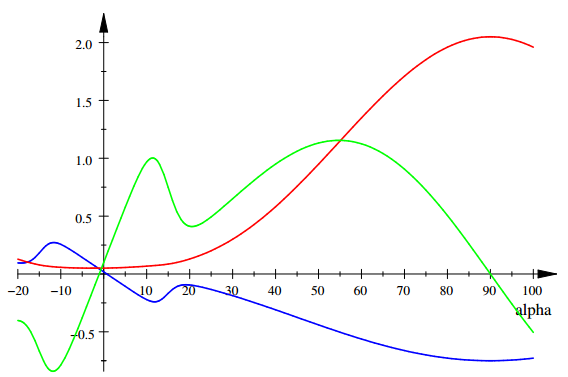
\includegraphics[width=300pt]{\IMAGEPATH /Data/lift_coeff}
	\caption{Skywalker X8 lift coefficient (green) vs angle of attack}
	\label{fig:lift}
\end{figure}

\subsection{Gyroscopic Effects}
\label{sec:gyro}
Angularion momentum: $H = I\omega$\\

Maximum motor speed $\omega = 800\times16.8\times\frac{2\pi}{60} = 1407.45rads^{-1}$\\

Prop Inertia $I = \frac{1}{12}\times M(L^2+B^2) = 1.16\times10^{-4}kgm^2$ (Overestimation as it assumes equally distributed mass, and constant width)\\

$\omega_p$ = Maximum servo rotation speed (procession) = $\frac{60^o}{0.11s} = 9.52rads^{-1}$\\

Using a small angle approximation $\Delta H = \omega_p \times\Delta t \times I \times \omega$\\ 

$\frac{dH}{dt} = \omega_p \times I \times \omega = M = 1.55Nm$\\

\begin{figure}[!ht]
	\centering
	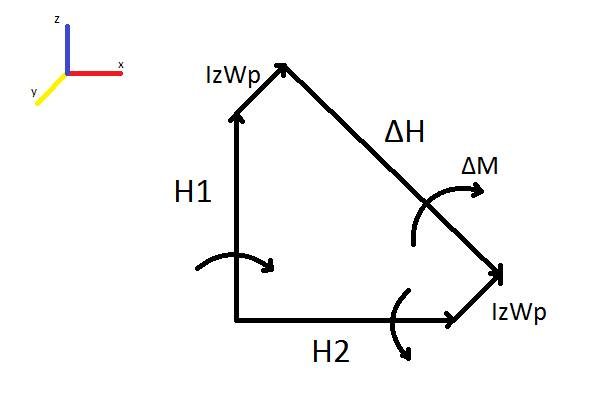
\includegraphics[width=200pt]{\IMAGEPATH /Diagrams/angular_momentum}
	\caption{Change in angular momentum during transition}
	\label{fig:momentum}
\end{figure}

Since the two front propellers are rotating in opposite directions, the change in angular momentum of each propeller during transition also acts in opposite directions, and the UAV is prevented from yawing (and possibly spinning out of control). This opposition also results in zero net force acting on the transition system.\\

\begin{figure}[!ht]
	\centering
	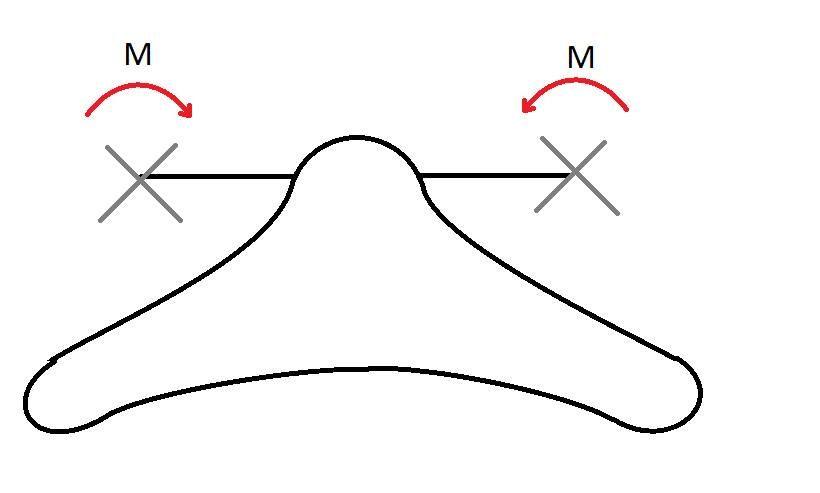
\includegraphics[width=100pt]{\IMAGEPATH /Diagrams/moments}
	\caption{Angular moments produced by aircraft motors}
	\label{fig:moments}
\end{figure}

However, the pole will experience a bending moment during transition. The maximum moment is exactly in the center of the front shaft, with magnitude $2M = 3.1Nm$. Since this is less than the moment on the front bar at hover ($2/3$ $\times M \times d = 9.156Nm$) the shaft should be capable of withstanding the gyroscopic effects.\\

\subsection{eCalc Modelling}
\label{sec:ecalc}
\begin{figure}[H]
	\centering
	\includegraphics[width=400pt]{\IMAGEPATH /Ecalc/eCalc1}
	\caption{Fixed-wing performance, 11 inch props}
\end{figure}
\begin{figure}[H]
	\centering
	\includegraphics[width=400pt]{\IMAGEPATH /Ecalc/eCalc2}
	\caption{VTOL performance, 11 inch props}
\end{figure}
\begin{figure}[H]
	\centering
	\includegraphics[width=400pt]{\IMAGEPATH /Ecalc/eCalc3}
	\caption{Fixed-wing performance, 12 inch props}
	\label{fig:fixed}
\end{figure}
\begin{figure}[H]
	\centering
	\includegraphics[width=400pt]{\IMAGEPATH /Ecalc/eCalc4}
	\caption{VTOL performance, 12 inch props}
	\label{fig:vtol}
\end{figure}
\begin{figure}[H]
	\centering
	\includegraphics[width=400pt]{\IMAGEPATH /Ecalc/eCalc7}
	\caption{Fixed-wing performance, 12 inch props, 3 batteries}
\end{figure}
\begin{figure}[H]
	\centering
	\includegraphics[width=400pt]{\IMAGEPATH /Ecalc/eCalc8}
	\caption{VTOL performance, 12 inch props, 3 batteries}
\end{figure}

\newpage

\subsection{3D Printed Models}
\label{sec:print}
\begin{table}[!htbp]
	\centering
	\caption{Modelling iterations for motor mounts}
	\begin{tabulary}{\textwidth}{|l|L|}
		\hline 
		\centering
		\raisebox{-\totalheight}{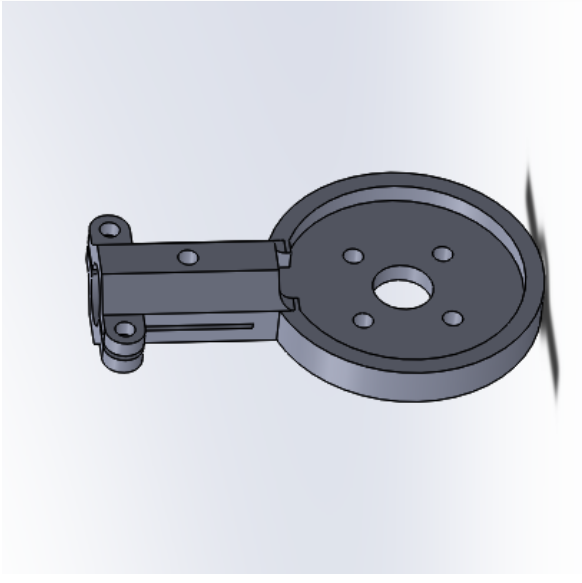
\includegraphics[width=200pt]{\IMAGEPATH Modelling/MotorMount1}} &
		\vspace{40pt} Initial designs of the motor mounts cased the motor in a small indent and had a hole through the center of the mount to carry wires. It was printed to give best fit to the pole while also using as little material as possible.
		It failed during testing at both 30\% and 100\% fill just before the start of the fillet between the pole and the motor. \\ 
		\hline 
		\centering
		\raisebox{-\totalheight}{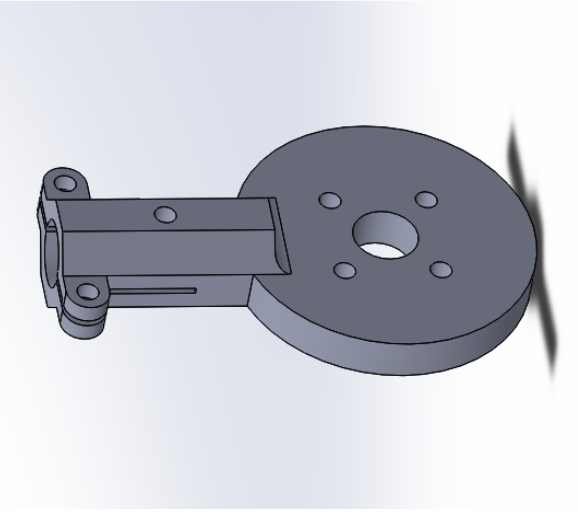
\includegraphics[width=200pt]{\IMAGEPATH Modelling/MotorMount2}} &
		\vspace{40pt} The second design fixed the weak point by not only extending the pole support into the flat mounting section, but also by removing the indent on the flat section.
		Another boost of strength was given by printing the mount flat, rather than upright, resulting in grains that ran orthogonal to previous lines of weakness and not parallel with them.
		When side screws were then tightened to increase friction, they split the mount due to the new weakness in the orientation. \\ 
		\hline 
		\centering
		\raisebox{-\totalheight}{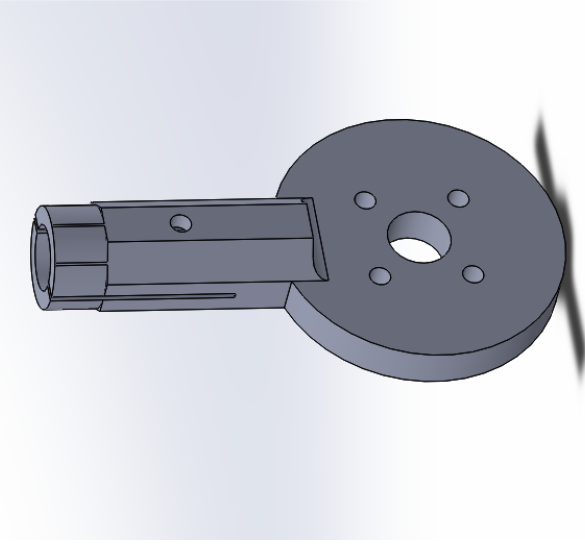
\includegraphics[width=200pt]{\IMAGEPATH Modelling/MotorMount3}} &
		\vspace{40pt} The current design for the motor mounts removed the side tabs that were meant to provide increased friction onto the motor pole. These were replaced by a rounded section in which a hose clamp is used to grip the mount to the pole. This design was printed on its side (round edge on the table) which was found to have the most strength in testing.\\ 
		\hline
	\end{tabulary} 
	\label{tab:3D_motor}
\end{table}

\newpage

\begin{table}[!htbp]
	\centering
	\caption{Modelling iterations for front mounts}
	\begin{tabulary}{\textwidth}{|l|L|}
		\hline 
		\centering
		\raisebox{-\totalheight}{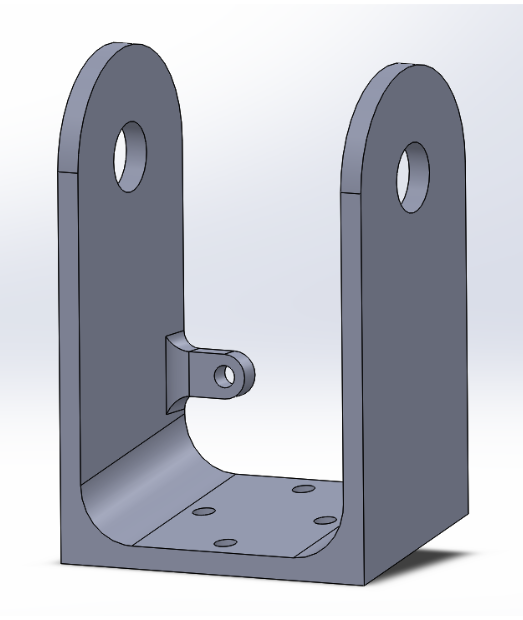
\includegraphics[width=160pt]{\IMAGEPATH Modelling/FrontMount1}} &
		\vspace{40pt} The initial design of the front pole mount was for the first hover tests that were planned. They fit within the recess in the front of the X8 with the carbon fibre rods fitting through to the outer sections of the plane. Screws at the back were initially used to give support.\\ 
		\hline 
		\centering
		\raisebox{-\totalheight}{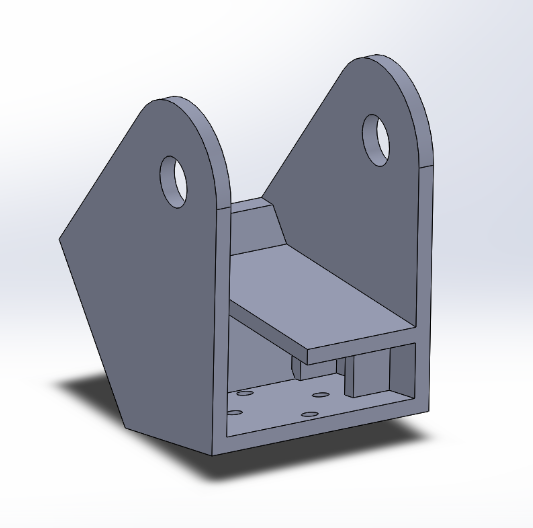
\includegraphics[width=160pt]{\IMAGEPATH Modelling/FrontMount2}} &
		\vspace{40pt} The second design was modified in order to fit the servo for the transition system. It was found that putting a servo within the mount increased strength and accuracy, and decreased vibrations through the shaft significantly.\\ 
		\hline
		\centering
		\raisebox{-\totalheight}{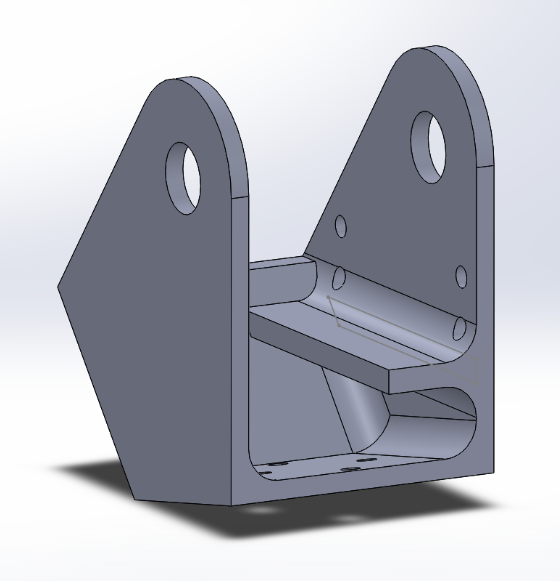
\includegraphics[width=160pt]{\IMAGEPATH Modelling/FrontMount3}} &
		\vspace{40pt} The third and final design included fillets for extra lateral strength. \\ 
		\hline 
	\end{tabulary} 
	\label{tab:front_mount}
\end{table}

\newpage

\begin{table}[!htbp]
	\centering
	\caption{Modelling iterations for back mounts}
	\begin{tabulary}{\textwidth}{|l|L|}
		\hline
		\centering
		\raisebox{-\totalheight}{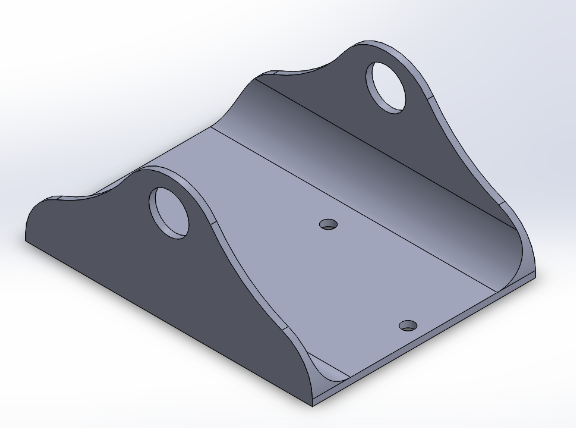
\includegraphics[width=160pt]{\IMAGEPATH Modelling/BackMount1}} &
		\vspace{40pt} The first back pole mount design was used on the Scorpion prototype. Initially, it also served as a basic front pole mount. The back servo was mounted external to the shaft using zip ties and screws, hence it was not very stable.  \\ 
		\hline 
		\centering
		\raisebox{-\totalheight}{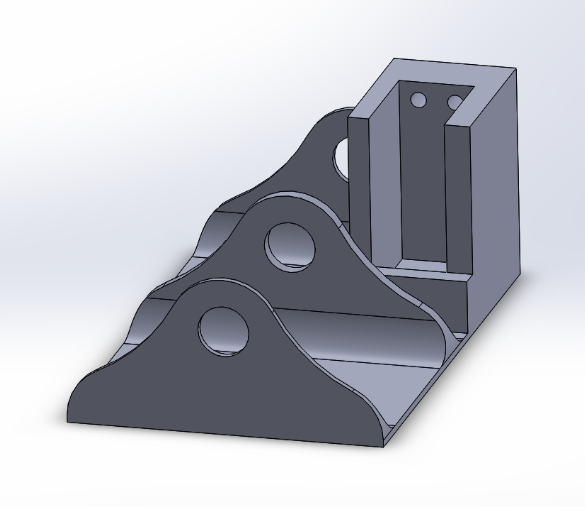
\includegraphics[width=160pt]{\IMAGEPATH Modelling/BackMount2}} &
		\vspace{40pt} Once the testing on the Scorpion prototype was complete, the mount was redesigned for the Dragonfly. This mount houses the servo, increasing stability and robustness. It also has 3 points of pole support in order to counter the moment and force created by the propeller.\\ 
		\hline 
	\end{tabulary} 
	\label{tab:back_mount}
\end{table}

\begin{table}[!htbp]
	\centering
	\caption{Gear, Legs and Front Ring Designs}
	\begin{tabulary}{\textwidth}{|l|L|}
		\hline
		\centering
		\raisebox{-\totalheight}{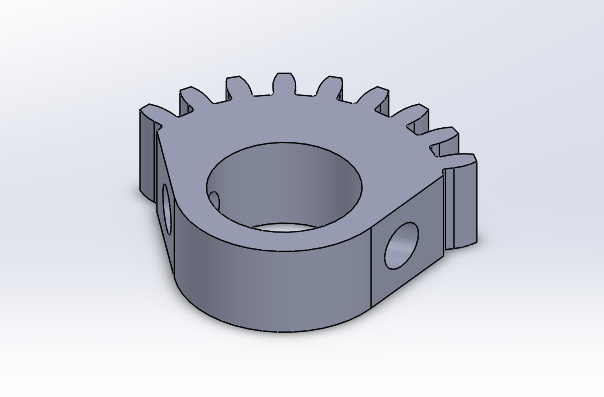
\includegraphics[width=160pt]{\IMAGEPATH Modelling/PoleGear}} &
		\vspace{30pt} The final design of the pole gear has holes to bolt into the shaft and is capable of 100 degrees of rotation. These are put on both rods attached to the aircraft, assisting with both transition in the front and the yaw mechanism in the back.  \\ 
		\hline 
		\centering
		\raisebox{-\totalheight}{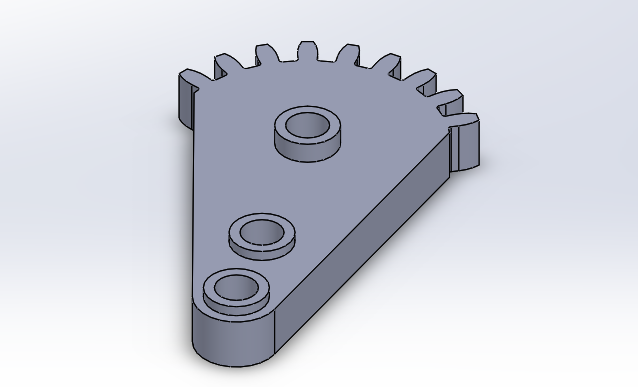
\includegraphics[width=160pt]{\IMAGEPATH Modelling/ServoGear}} &
		\vspace{30pt} The final servo gear was made to attach to the specific servo horn in 3 places. This allowed it to utilise the teeth of the servo, giving it very little slip.\\ 
		\hline 
		\centering
		\raisebox{-\totalheight}{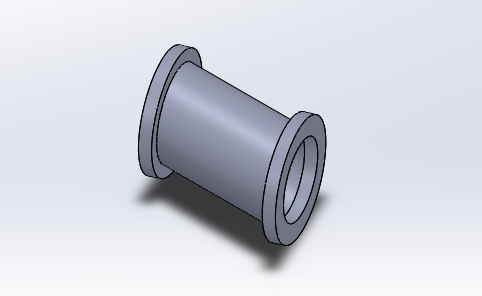
\includegraphics[width=160pt]{\IMAGEPATH Modelling/SideRing}} &
		\vspace{40pt} The side rings were used on the front shaft to provide an extra point of support for the front pole, and resulted in less friction between the foam and the carbon fiber rods. \\ 
		\hline 
		\centering
		\raisebox{-\totalheight}{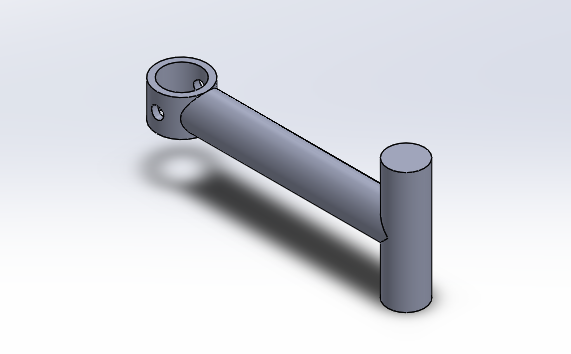
\includegraphics[width=160pt]{\IMAGEPATH Modelling/Leg}} &
		\vspace{20pt} The leg design for the Dragonfly was made to stabilise the roll rotation while on the ground in order to keep the front propellers safe. The design does not impede on the aerodynamic performance (as they rotate backwards during transition to fixed wing), nor does it impede on the back propeller which stays level while on the ground, and can safely rotate.\\ 
		\hline 
	\end{tabulary} 
	\label{tab:minor}
\end{table}